%%===========================================================%%
%%                                                           %%
%%                     EVENT SELECTION                       %%
%%                                                           %%
%%===========================================================%%


\newcommand{\itemm}{\item\hspace*{-5pt}.\hspace*{-1pt}~}

\chapter{Event selection}\label{chap:eventSelection}

Complete list of analysis cuts used for signal extraction is presented in Sec.~\ref{sec:listOfCuts}. Detailed description of each cut can be found in Sec.~\ref{sec:descriptionOfCuts}.

\section[List of cuts]{List of cuts\footnote{Some cuts (e.g.~\ref{enum:CutTpcTrks}) are decomposed to constituent sub-cuts. Cut is formed by the logical AND of all its sub-cuts.}}\label{sec:listOfCuts}
\begin{enumerate}[label=\textbf{C\arabic*},ref=C\arabic*]
 \itemm Exactly 1 primary vertex with TPC track(s) matched with hits in TOF.\label{enum:CutPrimVx}
 \itemm TPC vertex from~\ref{enum:CutPrimVx} is placed within $|z_{\textrm{vx}}|<100$~cm.\label{enum:CutZVx}
 \itemm Exactly 2 opposite-sign primary TPC tracks~(\ref{enum:TpcOppoSign}) of good quality and within high TPC acceptance region~(\ref{enum:TpcQualityCuts}) matched with hits in TOF~(\ref{enum:TpcTofMatched}).\label{enum:CutTpcTrks}
    \begin{enumerate}[label=\textbf{\theenumi.\arabic*},ref=\theenumi.\arabic*]
      \itemm Exactly 2 TOF-matched primary tracks,\label{enum:TpcTofMatched}
      \itemm Tracks are of opposite signs,\label{enum:TpcOppoSign}
      \itemm Both tracks satisfy criteria below:\label{enum:TpcQualityCuts}\\
      $|\eta|<1$,~~~~$p_{T}>0.2~\textrm{GeV}/c$,~~~~$\textrm{DCA}<2$~cm,~~~~$N_{\textrm{hits}}^{\textrm{fit}}\geq25$,~~~~$N_{\textrm{hits}}^{\textrm{dE/dx}}\geq15$,~~~~$N_{\textrm{hits}}^{\textrm{fit}}/N_{\textrm{hits}}^{\textrm{poss}}\geq0.52$,
    \end{enumerate}
 \itemm Exactly 1 RP track on each side of STAR central detector~(\ref{enum:RpOneTrkPerSide}) of good quality~(\ref{enum:RpQualityCuts}), with local angles consistent with the IP being the track origin~(\ref{enum:RpLocalAngles}), lying within fiducial region of high geometrical acceptance~(\ref{enum:RpFiducial}).\label{enum:CutRpTrks}
      \begin{enumerate}[label=\textbf{\theenumi.\arabic*},ref=\theenumi.\arabic*]
      \itemm RP tracks contain only track-points with at least 3 (out of 4) planes used in reconstrucion,\label{enum:RpQualityCuts}
      \itemm Local angles $[\textrm{mrad}]$ lie within $-1.2<\theta_{x}^{\textrm{RP}}<5.0$ and $1.5<|\theta_{y}^{\textrm{RP}}|<4.5$,\label{enum:RpLocalAngles}
      \itemm Exactly 1 track passing cuts \ref{enum:RpQualityCuts}-\ref{enum:RpLocalAngles} per side,\label{enum:RpOneTrkPerSide}
      \itemm Tracks passing cut~\ref{enum:RpOneTrkPerSide} lie within the $(p_{x},p_{y})$ region defined as\label{enum:RpFiducial}:~~~~~~$|p_{y}|>0.2~\textrm{GeV}/c$,\\[4pt]
      $(p_{x}/(\textrm{GeV}/c)+0.3)^{2}+(p_{y}/(\textrm{GeV}/c))^{2}<0.46^{2}$,~~~~~~~$(p_{x}/(\textrm{GeV}/c)-0.15)^{2}+(p_{y}/(\textrm{GeV}/c))^{2}<0.42^{2}$.
    \end{enumerate}
 \itemm Vertex $z$-positions measured in TPC and reconstructed from the difference of proton detection time in west and east RPs are consistent with each other within the resolution $|z_{\textrm{vx}}^{\textrm{TPC}}-z_{\textrm{vx}}^{\textrm{RP}}|<36$~cm.\label{enum:CutDeltaZVx}
 \itemm No signal in any tile of BBC-large (east or west) with $\textrm{ADC}>40$ and $\textrm{TDC}>100$.\label{enum:CutBbcLarge}
 \itemm Maximally 2 reconstructed TOF clusters $N^{\textrm{TOF}}_{\textrm{clstrs}}\leq 2$.\label{enum:CutTofClusters}
 \itemm Missing (total) momentum of TPC tracks and RP tracks $p_{T}^{\textrm{miss}}<75~\textrm{MeV}/c$.\label{enum:CutMissingPt}
 \itemm Particle (pair) identification:\label{enum:CutPid}\\
 \textbf{~~if~~} $n\sigma_{\textrm{pion}}^{\textrm{pair}}>3$ \textbf{~~\&~~} $n\sigma_{\textrm{kaon}}^{\textrm{pair}}>3$ \textbf{~~\&~~} $n\sigma_{\textrm{proton}}^{\textrm{pair}}<3$ \textbf{~~\&~~} $m^{2}_{\textrm{TOF}}>0.6~\textrm{GeV}/c^{2}~~\rightarrow~~pp$\\%
\textbf{elif~~} $n\sigma_{\textrm{pion}}^{\textrm{pair}}>3$ \textbf{~~\&~~} $n\sigma_{\textrm{kaon}}^{\textrm{pair}}<3$ \textbf{~~\&~~} $n\sigma_{\textrm{proton}}^{\textrm{pair}}>3$ \textbf{~~\&~~} $m^{2}_{\textrm{TOF}}>0.15~\textrm{GeV}/c^{2}~~\rightarrow~~KK$\\%
\textbf{elif~~} $|n\sigma_{\textrm{pion}}^{\textrm{trk1}}|<3$ \textbf{~~\&~~} $|n\sigma_{\textrm{pion}}^{\textrm{trk2}}|<3~~\rightarrow~~\pi\pi$\\%
\textbf{else~~} event rejected.
\end{enumerate}

\section{Description of cuts}\label{sec:descriptionOfCuts}
\subsection{(\ref{enum:CutPrimVx},\ref{enum:CutZVx})~Primary vertex}
Bla bla
\subsection{(\ref{enum:CutTpcTrks})~TPC tracks}
\subsection{(\ref{enum:CutRpTrks})~RP tracks}
\subsection{(\ref{enum:CutDeltaZVx})~TPC-RP \texorpdfstring{$z$}{z}-vertex matching}
\subsection{(\ref{enum:CutBbcLarge})~BBC-large signal veto}
\subsection{(\ref{enum:CutTofClusters})~TOF clusters limit}
\subsection{(\ref{enum:CutMissingPt})~Exclusivity cut (missing \texorpdfstring{$p_{T}$}{pT} cut)}
\subsection{(\ref{enum:CutPid})~Particle identification}

In addition to information from the TPC we use time of hit detection in the barrel TOF subsystem. From the simple algebra describing relation between track lengths, momenta and times of hit detection one can derive formula for the squared mass of two particles, assuming that their masses are equal (particles are of the same type):

%---------------------------
\begin{figure}[ht!]
\centering%
\parbox{0.29\textwidth}{%
  \centering%
  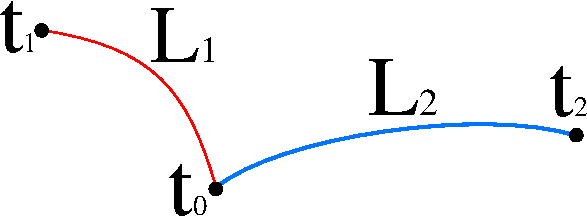
\includegraphics[width=\linewidth]{graphics/eventSelection/TofScheme.pdf}\label{fig:tofScheme}
}%
\quad\quad%
\parbox{0.655\textwidth}{%
    \caption[Scheme of two central tracks with common vertex, hitting cells in TOF detector.]{Scheme of two central tracks of lengths $L_{1}$ and $L_{2}$, produced in common vertex in moment $t_{0}$, hitting cells in TOF detector in moments $t_{1}$ and $t_{2}$.}
}%

\end{figure}
%---------------------------

\begin{equation}
 \left\{\begin{array}{l}%
 t_{1}-t_{0} = L_{1}\sqrt{1+\frac{m_{1}^{2}}{p_{1}^{2}}}, \\[3pt]
 t_{2}-t_{0} = L_{2}\sqrt{1+\frac{m_{2}^{2}}{p_{2}^{2}}},
\end{array}\right.%
\end{equation}

\begin{equation}
 \Delta t = t_{1}-t_{2} = L_{1}\sqrt{1+\frac{m_{1}^{2}}{p_{1}^{2}}} - L_{2}\sqrt{1+\frac{m_{2}^{2}}{p_{2}^{2}}}.
\end{equation}

\[\textrm{Assuming}~m_{1}=m_{2}=m~~\rightarrow~~m^{2}~\textrm{from quadratic eq.}\]
Parameters of the quadratic equation whose solution is suqared mass and the final formula for $m^{2}_{\text{TOF}}$ are given below:
\begin{equation}
\mathcal{A}= -2\frac{L^2_1L^2_2}{p^2_1p^2_2}+\frac{L^4_1}{p^4_1}+\frac{L^4_2}{p^4_2},
\end{equation}
\begin{equation}
\mathcal{B}=-2L^2_1L^2_2\left({\frac{1}{p^2_1}} + {\frac{1}{p^2_2}}\right)+\frac{2L^4_1}{p_1^2}+\frac{2L^4_2}{p_2^2}-2\left(\Delta t\right)^2\left(\frac{L^2_1}{p_1^2}+\frac{L^2_2}{p_2^2}\right),
\end{equation}
\begin{equation}
\mathcal{C}=\left(\Delta t\right)^4-2\left(\Delta t\right)^2\left(L^2_1+L^2_2\right)+L^4_1+L^4_2-2L^2_1L^2_2,
\end{equation}
\begin{equation}
 \label{eq:mSquared}
m^{2}_{\textrm{\tiny TOF}} = \frac{-\mathcal{B}+\sqrt{\mathcal{B}^2-4\mathcal{A}\mathcal{C}}}{2\mathcal{A}}.
\end{equation}


\section{Working point for cuts~\ref{enum:CutBbcLarge}, \ref{enum:CutTofClusters} and \ref{enum:CutMissingPt}}

\begin{tabulary}{\textwidth}{LLL}
\begin{equation}\label{eq:significance}\hspace*{-10pt}
	\textrm{Significance} = \frac{N_{\textrm{signal}}^{\textrm{cut}}}{\sqrt{N_{\textrm{signal}}^{\textrm{cut}} + N_{\textrm{bkgd}}^{\textrm{cut}}}},
\end{equation}~~~~~~~~~~~~~~~~~&
\begin{equation}\label{eq:efficiency}\hspace*{-10pt}
	\textrm{Efficiency} = \frac{N_{\textrm{signal}}^{\textrm{cut}}}{N_{\textrm{signal}}^{\textrm{no~cut}}},
\end{equation}~~~~~~~~~~~~~~&
\begin{equation}\label{eq:purity}\hspace*{-9pt}
	\textrm{Purity} = \frac{N_{\textrm{signal}}^{\textrm{cut}}}{N_{\textrm{signal}}^{\textrm{cut}}+N_{\textrm{bkgd}}^{\textrm{cut}}},
\end{equation}~~~~~~~~~~~~~~~
\end{tabulary}


%---------------------------
\begin{figure}[hb]
\centering
\parbox{0.4725\textwidth}{
  \centering
  \begin{subfigure}[b]{\linewidth}
                \subcaptionbox{\label{fig:SignificanceVsEff}}{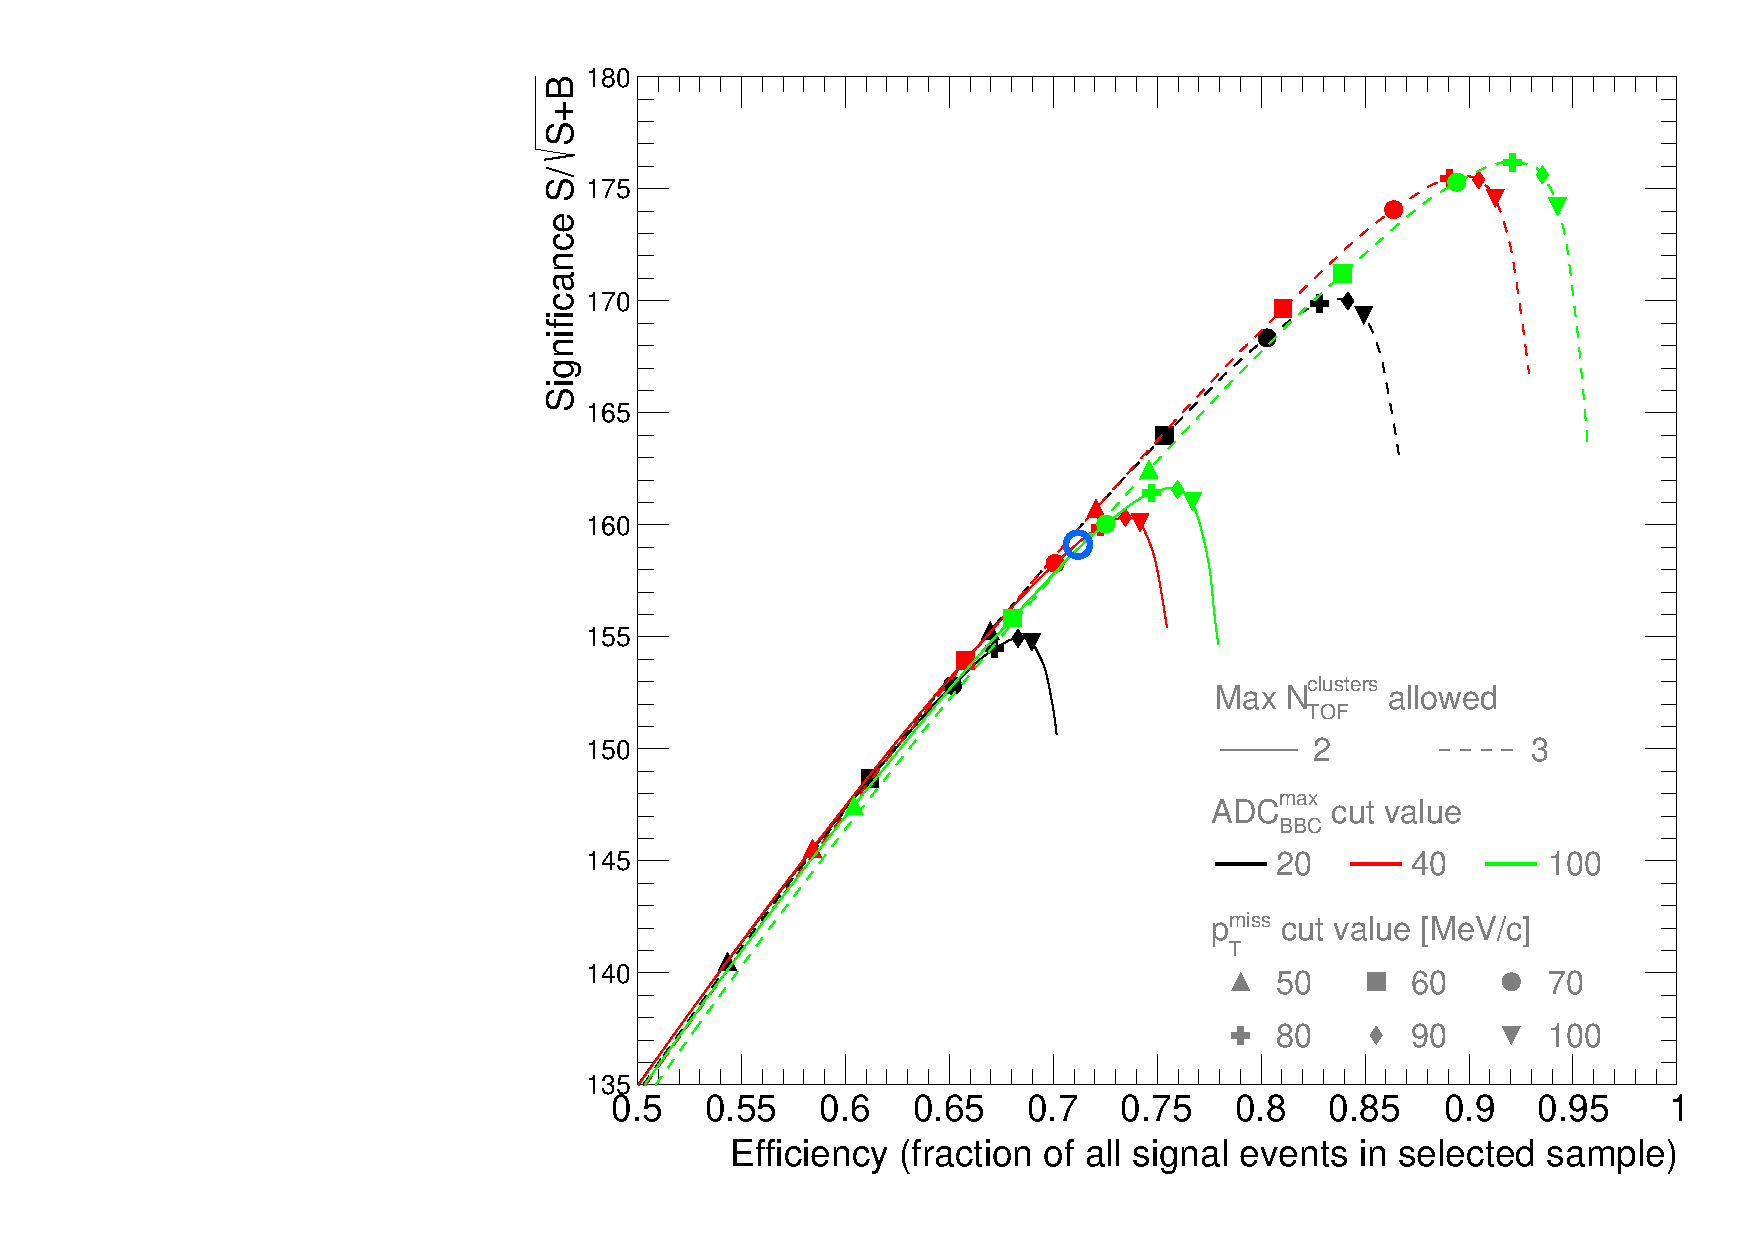
\includegraphics[width=\linewidth]{graphics/eventSelection/SignificanceVsEfficiency_pTmiss.pdf}}
  \end{subfigure}\\
  \begin{subfigure}[b]{\linewidth}\addtocounter{subfigure}{1}
                \subcaptionbox{\label{fig:EffVsBkgdFrac}}{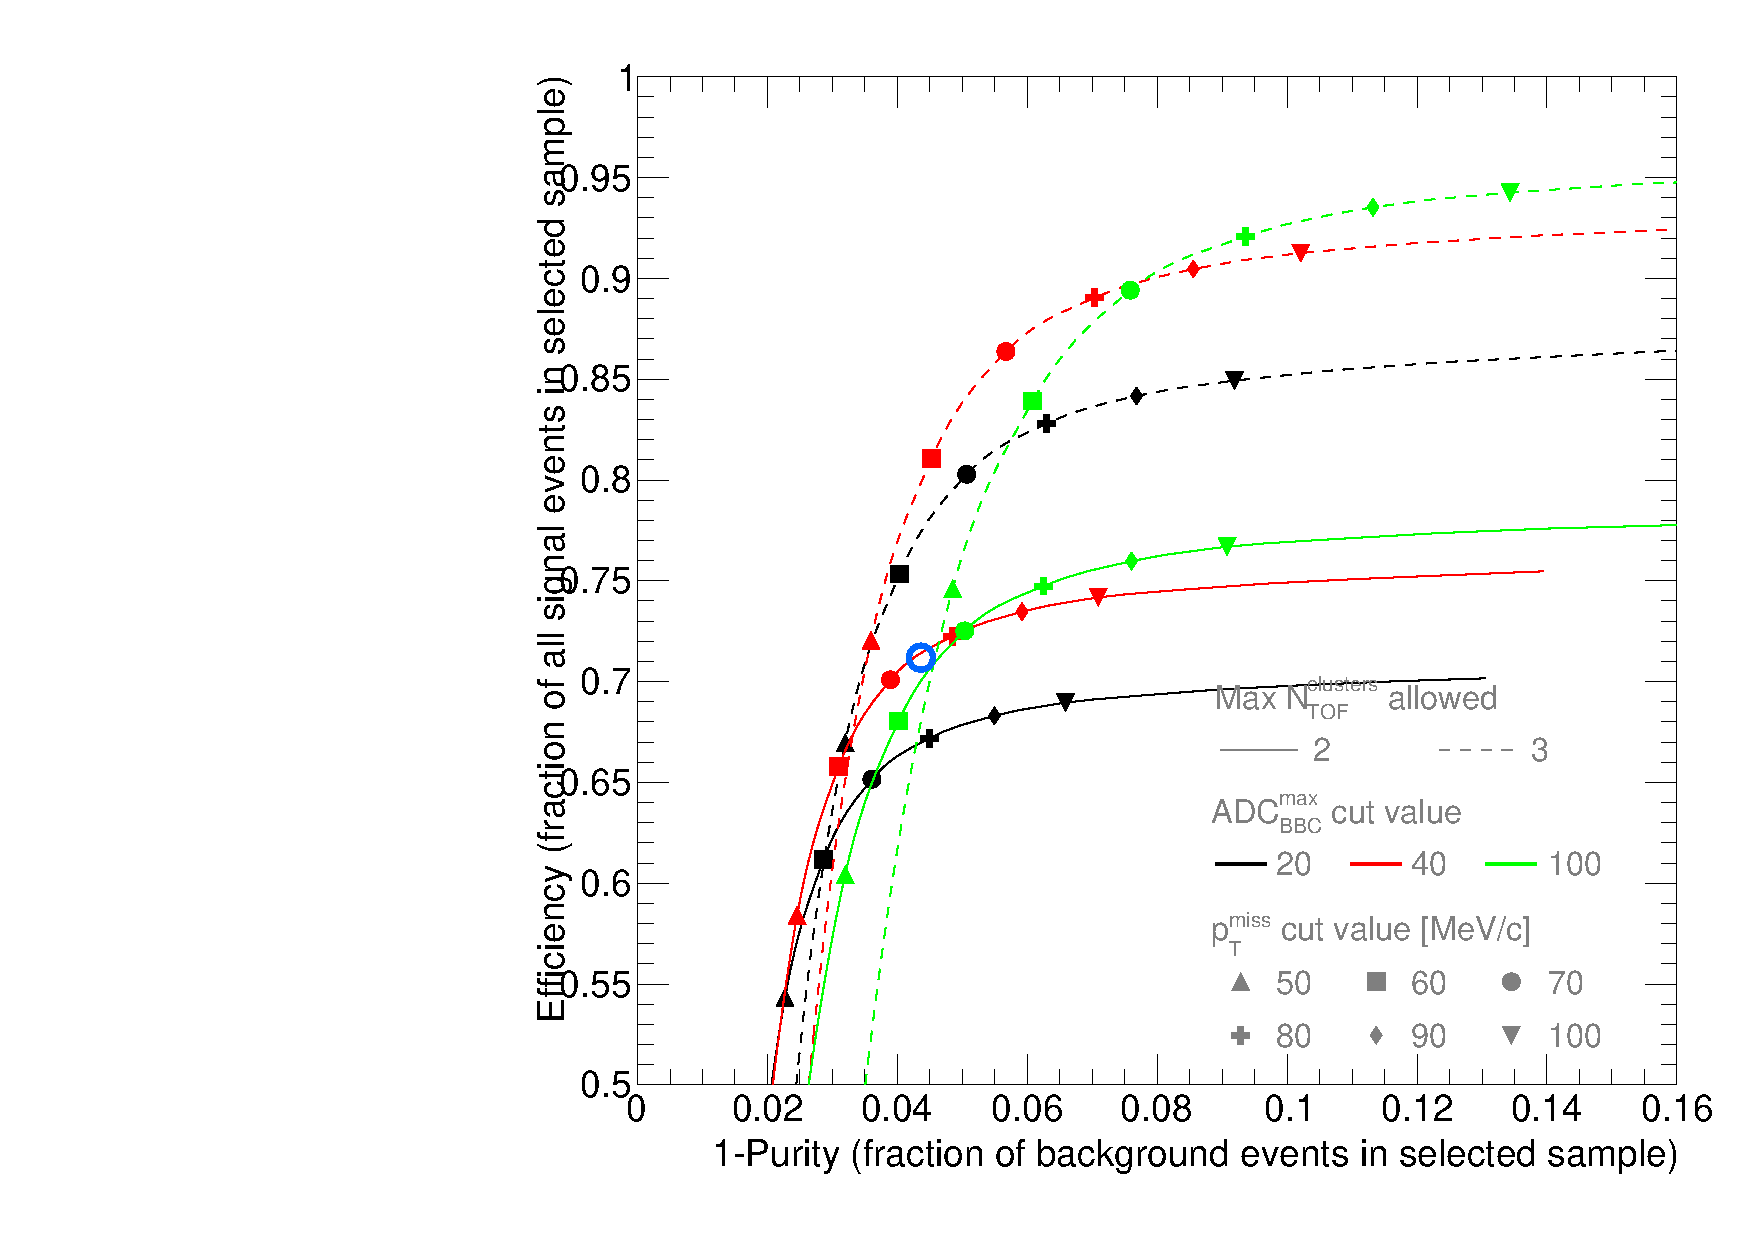
\includegraphics[width=\linewidth]{graphics/eventSelection/ROC_pTmiss.pdf}}
  \end{subfigure}
}%
\quad%
\parbox{0.4725\textwidth}{
  \centering
  \begin{subfigure}[b]{\linewidth}\addtocounter{subfigure}{-2}
                \subcaptionbox{\label{fig:SignificanceVsBkgdFrac}}{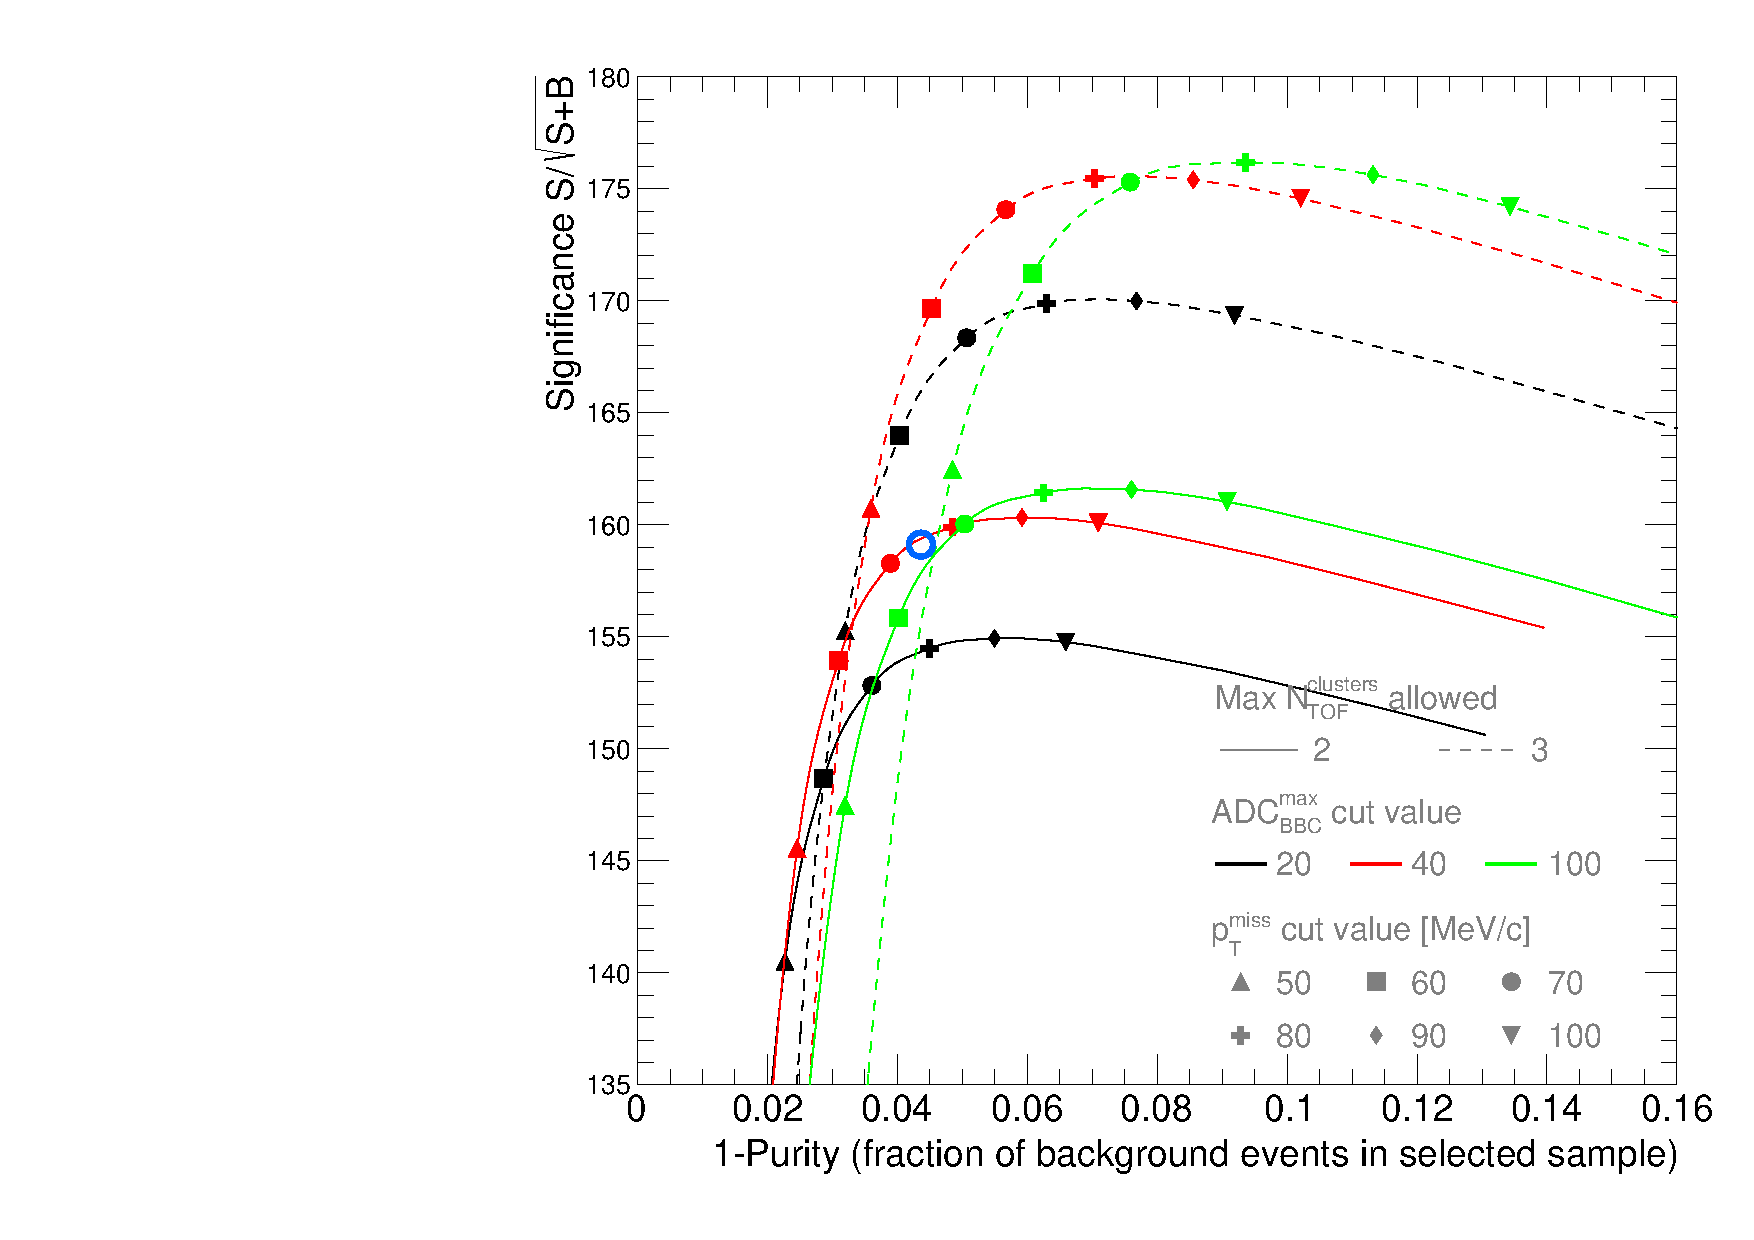
\includegraphics[width=\linewidth]{graphics/eventSelection/BkgdFractionVsEfficiency_pTmiss.pdf}}
  \end{subfigure}\\
  \begin{minipage}[t][1.042\linewidth][t]{\linewidth}\vspace{10pt}
    \caption[Relation between $\pi^{+}\pi^{-}$ significance, efficiency and purity vs. thresholds in cuts~\ref{enum:CutBbcLarge}, \ref{enum:CutTofClusters} and \ref{enum:CutMissingPt}]{Relation between $\pi^{+}\pi^{-}$ signal significance and efficiency (\ref{fig:SignificanceVsEff}), significance and purity (\ref{fig:SignificanceVsBkgdFrac}), and efficiency and purity (\ref{fig:EffVsBkgdFrac}) as a function of cut thresholds in BBC-large veto (\ref{enum:CutBbcLarge}), TOF cluster limit (\ref{enum:CutTofClusters}) and exclusivity cut (\ref{enum:CutMissingPt}). Lines show forementioned relations with changing $p_{T}^\textrm{miss}$ cut whose some specific values are indicated with different markers. Color denotes ADC threshold in BBC-large veto (black, red or green). Style of line (solid or dashed) denotes $N^{\textrm{TOF}}_{\textrm{clstrs}}$ limit. Working point considered optimal is marked with opened blue circle.}\label{fig:workingPoint}
  \end{minipage}
}%

\end{figure}
%---------------------------


\section{Signal per integrated luminosity}

\section{Cut flow}\label{sec:cutFlow}